\documentclass[conference, 10pt]{IEEEtran}

%% IEEE CNS addition:
\makeatletter
\def\ps@headings{%
	\def\@oddhead{\mbox{}\scriptsize\rightmark \hfil \thepage}%
	\def\@evenhead{\scriptsize\thepage \hfil \leftmark\mbox{}}%
	\def\@oddfoot{}%
	\def\@evenfoot{}}
\makeatother
\pagestyle{empty}
\IEEEoverridecommandlockouts
%\IEEEpubid{\makebox[\columnwidth]{978-1-5386-2487-6/17/\$31.00~\copyright~2017 IEEE \hfill} \hspace{\columnsep}\makebox[\columnwidth]{ }}


%\usepackage[top=.75in,bottom=1in,left=.825in,right=.825in]{geometry}
%\usepackage[margin=1in]{geometry}
%\usepackage[hidelinks]{hyperref}
\usepackage{graphicx}
\let\proof\relax
\usepackage{amsmath}
\let\endproof\relax
\usepackage{amsthm}
\usepackage{amsfonts}
\usepackage{subcaption}
\usepackage{algorithm,caption}
\usepackage{algpseudocode}
\usepackage[normalem]{ulem}
\usepackage{booktabs}

\begin{document}
	
	\title{An Investigation into the use of Reinforcement Learning for Enhanced Queue Stability in RED Gateways \vspace{-2ex}}
	\author{\IEEEauthorblockN{Vignesh Pagadala\IEEEauthorrefmark{1}, Joseph Gersch \IEEEauthorrefmark{2}}
	\IEEEauthorblockA{Department of Computer Science,
		Colorado State University\\
		Fort Collins, CO, 80523, USA\\
		Email:
		\IEEEauthorrefmark{1}Vignesh.Pagadala@colostate.edu,
		\IEEEauthorrefmark{2}Joe.Gersch@colostate.edu}
	\vspace{1ex}}
	\maketitle
	
	\begin{abstract}
	Despite being a well-established congestion-avoidance scheme in packet-switched networks, there happens to be a general reluctance amongst network administrators in implementing Random Early Detection (RED) in their network gateways. This is due to the presence of several adjustable parameters associated with RED, whose values are to be determined by the network administrators themselves. There happens to be no known methods which espouse on how to manually set these values to achieve peak network performance. To circumvent this problem, several studies have relied on automating this procedure, using feedback about the performance over discretized time intervals, and information regarding the state of the network to arrive at an optimum solution. In this work we shall adopt a reinforcement-learning-based approach to arrive at the optimal values of the control parameters, more specifically on tuning the parameters Qmax and Qmin. We then simulate a network environment using a discreet-events simulator. After several learning iterations, the results obtained demonstrated that the learning methodology could indeed converge upon reasonable values for Qmax and Qmin. However, these values are limited to a given network behavior, and will not be applicable to a highly dynamic network (the implications of which will be discussed in the paper). In any case, the values suggested by this approach result in good queue stability, minimal packet drops and high link utilization.        
	\end{abstract}

\section{Introduction}
\label{sec:intro}

\subsection{Random Early Detection and its Significance}
\label{sec:intro:significance}

RED is a congestion-avoidance methodology proposed by Floyd et al. \cite{floyd1993random} which suggests the use of Active Queue Management (AQM) techniques in network gateway buffers in order to mitigate congestion. Conventionally, gateways use a suitably-sized network buffer in order to be capable of absorbing momentary bursts in traffic. However, certain situations might involve sources sending packets at a rate much higher than what the outbound link of the gateway is capable of handling. In such situations, the buffer gets rapidly filled up to capacity, and can no longer accept any more incoming packets. This would cause every arriving packet to get dropped. This rather simplistic approach to queue management is referred to as the 'Tail Drop' methodology, wherein, gateways drops all packets after the buffer is full. 

Though this methodology would work with respect to notifying senders that their sending rate is too high, it would significantly bring down the throughput of the network, measured in terms of link utilization. As the buffer gets filled, and every packet gets dropped, the senders observe their packets getting dropped and every sender may simultaneously decide to perform multiplicative decrease of their congestion windows sizes. This global synchronization might be disastrous to network performance, as link utilization would decrease drastically, and it might only have been necessary for a few of the senders to reduce their congestion window sizes (in order to prevent congestion at the gateway). Therefore, RED proposes to inform the senders of incipient congestion at the gateway way before actual congestion takes place. This is done through the following strategy. 

Floyd et al. propose maintaining two different threshold values for the length of the queue - $Q_{max}$ and $Q_{min}$. $Q_{max}$ represents the maximum threshold of the queue length. If the queue length exceeds this threshold, every incoming packet after this is dropped. $Q_{min}$ represents the minimum threshold. If the queue length exceed this minimum threshold, every packet is dropped with a certain probability. This probability value is defined by a probability distribution which is dependent on the queue length, and varies linearly (increasing with increasing queue length). Floyd et al. also provide information on how to calculate the queue length, and probability distribution. 

This technique is undoubtedly much better than tail-drop wherein, the problems associated with global synchronization (global backoff of congestion window sizes) are circumvented. This solution also happens to be capable of maintaining low queue sizes, which allows for gateways buffers to be used for the actual purpose that they are in place for - mitigating bursty traffic. RED is a widely-known AQM scheme \cite{chen2011self}, and despite its well-understood benefits, there are issues with respect to setting the parameters involved in order to maximize throughput. It is clear that the values of the control parameters are different for different network scenarios, and there happens to be no clear and definitive formula which can come to the aid of network administrators.  

\begin{figure*}[t]
	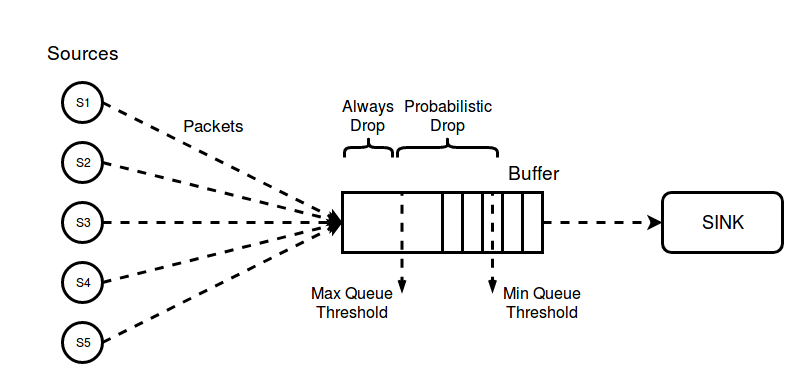
\includegraphics[width = \linewidth]{Dg1.png}
	\caption{RED Algorithm}
	\label{fig:1}
\end{figure*}

\subsection{Control-Parameter Tuning}
\label{sec:intro:cprtuning}

There are various parametric configurations possible in RED. From the original work of Floyd et al. these parameters are the maximum queue length threshold ($Q_{max}$), the minimum queue length threshold ($Q_{min}$), weight associated with the average queue length calculation ($w_q$) and the maximum drop probability ($p_{max}$). Finding the right parameter-set is important to strike a good balance between high network link utilization and low packet drops. From a study performed on different RED configurations by Feng et al. \cite{feng1999self}, very assertive packet drop/marking resulting in a high level of congestion notifications would minimize packet drops, but causes very low link utilization, and minimal congestion notifications through packet marking would ensure high link utilization through high congestion window values, but causes lots of packet drops.   



\subsection{Established Approaches}
\label{sec:intro:currentapp}
Several mechanisms have been proposed to find a workaround to this problem. Many of them involve automating the parameter-setting procedure, based on information about the network state. In the proposition by Feng et al. \cite{feng1999self}, the average queue length is monitored periodically, and depending on where the value happens to be oscillating at, they infer as to the whether the RED mechanism is too assertive or too liberal (assertive if $Q_{avg}$ oscillates around $Q_{min}$, and liberal if $Q_{avg}$ oscillates around $Q_{max}$). Based on this information, one of the control parameters, the value of maximum drop probability $p_{max}$, is continually varied. Results show $p_{max}$ increasing with increasing number of connections, and vice versa, automatically. Chen et al. \cite{chen2011self}, not only try varying the maximum drop probability $p_{max}$, but also the weight of the average queue length calculation $w_q$. According to their analysis, queue stability is mathematically dependent on certain values of $p_{max}$ and $w_q$, and they tune these values based on this mathematical dependency. Their results indicate that the queue length is indeed stable compared with other AQM measures. 

Zhani et al. \cite{zhani2007alpha_} propose the use of $\alpha$-SNAFQM, wherein, they try to predict how the network traffic might behave in future using a neurofuzzy prediction technique, and accordingly tune the RED parameters. Masoumzadeh et al. \cite{masoumzadeh2011fql} propose FQL-RED, where they use fuzzy Q-learning to optimize RED parameters based on network status. Both these previous works show much better improvements over conventional RED, and at the same time maintain the original principles of RED intact. Misra et al. \cite{misra2010random} diverge from this trend by using a learning-automata like solution to modify the working of RED, bypassing the parameter usage. This method once again shows considerable improvements over the original RED algorithm. All these methods so far imply using some information about network flows to work out a solution. However, in the work by Jacobson et al. \cite{jacobson1999red}, they propose this auto-tuning simply by looking at the bandwidth of the output link, and arrive at an optimal value of $p_{max}$. This solution works successfully with a broad range of network characteristics.   

\subsection{Hypothesis}
\label{sec:intro:hypothesis}

In most of the work done in trying to automate RED parameterization, we can observe two classes of approaches. One class of approaches maintain the fundamental principles of RED, but do not comply with the exact specification, thereby working their way around the parameters involved. Another class of approaches actively involve the use of these parameters, and try to play the game by the rules (by modifying parameters based on network characteristics, and so on). Furthermore, the parameters chosen to be tweaked in most cases appears to be $p_{max}$, or $p_{max}$ and $w_q$. Masoumzadeh et al. \cite{masoumzadeh2011fql}, in their work, do try to work with $Q_{max}$ and $Q_{min}$. However, they do this in conjunction with trying to vary the other two parameters as well ($p_{max}$ and $w_q$). 

In their work, Floyd et al. \cite{floyd1993random} suggest an upper and lower bound for $w_q$, and provide a ``rule of thumb" for setting $Q_{max}$ and $Q_{min}$, where it is implied to set $Q_{max}$ to twice the value of $Q_{min}$, which is what most network administrators follow. In most of the background work, it is not clear if any one or two of the parameters are more sensitive, and have a greater influence on network performance than the other parameters. One question that might come up would be, if we can perform better than conventional RED using only a subset of the four control-parameters which have not been looked at the in the previous work - $Q_{max}$ and $Q_{min}$. In this work, we shall try to obtain the optimal values of $Q_{max}$ and $Q_{min}$ by looking at the network state, and observe the results. 

The problem domain also appears to be the perfect use-case for applying a machine learning method as so many of the other works described above have done. Reinforcement Learning intuitively appears to be a good tool for the job, owing to the discretized nature of network traffic. Furthermore, network characteristics in most cases are retained over periods of time, and may be dynamic over different periods, which would allow us to 'learn' this nature, and harness this knowledge to find optimal control parameter values (which would be done over each period). Using this as a starting point, in this work, we perform an exploratory study on using Reinforcement Learning techniques to arrive at optimal values of the control parameters $Q_{max}$ and $Q_{min}$. A discreet-events simulator is used to simulate the network characteristics, and we use Q-Learning to generate control parameter values for fixed network characteristics. Results showed that this methodology does indeed provide max and min threshold values that perform better than what a network administrator would have set manually (using Floyd et al.'s recommendations). However, though we show a comparative improvement, this method does not indicate if the final values are definitively the most optimal, owing to the probabilistic drops, and dynamic nature of networks in general.    

\subsection{Paper Outline}
\label{sec:intro:outline}
The organization of the subsequent sections of the paper is described as follows. Section \ref{sec:back} elaborates on a detailed description of the RED configuration parameters, queue length calculation, reinforcement learning concepts and the simulation methodology. Section \ref{sec:prop} provides a detailed description on the design of the solution, and algorithm to be followed. Section \ref{sec:analysis} shows the results obtained using simulations, and a comparison between manual setting, and using the auto-generated values. Section \ref{sec:conc} summarizes the contributions made in this work and section \ref{sec:future} indicates the direction in which this project could be extended in future. 
 

\section{Background}
\label{sec:back}
In this section, we shall look into different aspects of RED, a detailed view of the control parameters available at our disposal, and what they imply. We will also decide on a proper queue length calculation methodology, how reinforcement learning works and a brief overview of the simulation methodology. 
\subsection{RED Configuration}
\label{sec:back:ngacpm}

\subsubsection{Queue Length Calculation}
\label{sec:back:ngacpm:elements}
Before we get into a description of the control parameters involved, it is necessary to establish a suitable queue length calculation methodology. We have to remember here that the queue's length ascertains what actions are triggered such as drop or probabilistic drop, so it is important that we resolve this before moving ahead. We can choose to have a length calculation which is very dynamic, or has lesser variation over time, but captures the overall direction in which the buffer state is moving towards (increasing or decreasing congestion).

The following options are available at our disposal (based on details espoused in \cite{floyd1993random}):
\begin{itemize}
    \item Instantaneous queue length value:
    
    Choosing the instantaneous queue length is not a good idea since this would cause large variations, and the algorithm would be too sensitive to short term bursts \cite{floyd1993random}.  
    \item Exponential Weighted Moving Average:
    
    Floyd et al \cite{floyd1993random} have suggested the use of a lowpass-filter, or EWMA, to calculate the average weight. This would imply average queue length calculation using the following:
    $$avg = (1 - w_q)*avg+w_qQ$$
    where $w_q$ represents the queue length calculation weight and $Q$ is the instantaneous queue length. This implies that, a lower value of $w_q$ would correlate with a softer variation in $avg$, which is desirable. 
    
\end{itemize}
\subsubsection{Control Parameters}
\label{sec:back:ngacpm:rel}

As indicated before, the various control parameters available at our disposal are:

\begin{itemize}
    \item $p_{max}$ - Maximum drop probability. The drop-probability distribution would vary depending on $p_{max}$ as follows \cite{floyd1993random}:
    $$p_b = p_{max} * (avg - Q_{min})/(Q_{max} - Q_{min})$$
    \item $w_q$ - The weight associated with queue length calculation described above.
    \item $Q_{max}$ - Maximum queue length threshold, after which all packets are dropped.
    \item $Q_{min}$ - Minimum queue length threshold, after which packets undergo probabilistic drop. 
\end{itemize}

\subsection{Reinforcement Learning}
\label{sec:back:prev}
Reinforcement Learning is a machine learning paradigm, where, the algorithms are fed with a set of states and actions, and depending on what goals are desired, different state-action pairs are assigned a reward or punishment, which motivates the algorithm to proceed in a particular direction. For example, in a game of Tic-Tac-Toe, a state could be described with a 3 X 3 array, with different values for the Xs and Os. Each one of these states are in-turn associated with possible sets of actions which the algorithm can take from a particular state. The action with the highest reward will always be picked by the algorithm, and this would be an action which would lead it to the goal state from that given state. These reward values are in turn populated by several 'learning' iterations. 

In this work, we shall make use of Q-Learning. A Q function essentially provides us a value for a given state, and an action from that state. This Q function can be represented in the form of a Q-table. The idea is to iteratively explore, and observe sets of 'SARSA' which are $s_t, a_t, r_{t+1}, s_{t+1}, a_{t+1}$ (state, action, reinforcement, next state, next action). Q values could either be updated using Monte-Carlo updates (average of all reinforcements) or Temporal-Difference updates. In this work, we use Temporal-Difference updates in order to prevent excessive fluctuation in the Q values. 

$$Q(s_t,a_t) = Q(s_t,a_t) + \rho (r_{t+1} + Q(s_{t+1},a_{t+1}) - Q(s_t,a_t))$$
where $\rho$ represents the learning rate. We can control how focused the learning algorithm is initially (how much it tends to choose a 'greedy' move i.e. a move with a greatest reward) using the Epsilon Decay Factor. A value of 1 would encourage more random move selections, and slowly decays this to 0 with increasing iterations. 

\subsection{Discreet-Events Simulation}
\label{sec:back:discreet}
For simulating the network environment, in this work, we make use of a discreet events simulator package put together by Grotto Networking \cite{grotto} using SimPy. This package consists of the following sets of classes using which the simulation can be constructed:
\begin{itemize}
    \item Packet: Class which represents a packet. 
    \item PacketGenerator: Generates packets. Allows us to specify the congestion window at each source, to vary the rate at which packets are sent toward a particular destination.
    \item PacketSink: Used to receive packets and also to record their time of arrival.
    \item SwitchPort: Used to simulate the buffer. Allows us to specify the buffer capacity and maximum outbound link service rate.
    \item PortMonitor: Class used to monitor the buffer, and allows us to see information such as queue lengths over discreet time intervals.
\end{itemize}

\section{Methodology}
\label{sec:prop}
In this section, we shall propose the design guidelines of our reinforcement learning methodology, how we measure performance and the simulation architecture.

\subsection{Performance Measure}
\label{sec:prop:indexing}
Before we delve into the reinforcement learning part, it is necessary to decide on a good performance measure. After all, reinforcement learning requires a suitable goal state to converge upon. We use the following features to measure performance:
\begin{itemize}
    \item Source Congestion Window Size ($CWND$): This measure is a good indicator of total network link utilization. This is computed as the total congestion window sizes of all sources in the network at the end of the testing time interval. High value of $CWND$ would imply that sources are maximizing their bandwidth usage. Higher values of $CWND$ are better.
    \item Total number of packets dropped ($DROP$): Measured as the total number of packets dropped over the testing time interval.
    \item Average queue length stability ($STD$): This is measured by calculating the standard deviation of average queue length values over the testing time interval.
\end{itemize}

At first glance, it seems intuitive to use just $STD$ to measure performance. However, this is not something that would work successfully with the reinforcement learning approach. We shall elaborate on the reinforcement learning part in later sections. But if we use only $STD$, then the ideal goal state would be a standard deviation of zero. Training the reinforcement learning algorithm this way causes it to behave erratically, and drop every packet. Figure \ref{fig:queuestab} shows this behavior.


\begin{figure}[ht!]
	\centering
	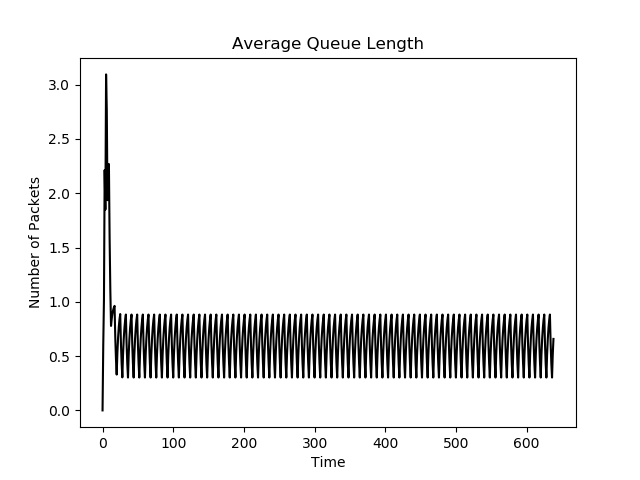
\includegraphics[width = 90mm]{QueueStab1.png}
	\caption{Using only queue stability as a performance measure is not a good idea. As can be observed in this plot, the algorithm sets the parameters in such a way that every packet gets dropped. This causes the queue length to be very stable (within 1 packet), but it is not desirable behavior.}
	\label{fig:queuestab}
\end{figure}

Therefore, it is essential to use $DROP$ and $CWND$ in conjunction with $STD$ in order to obtain desirable behavior, which in turn would be a good balance between high link utilization, and low packet drops. 

\subsection{Q-Learning}
\label{sec:prop:accreq}
How can we translate this into a reinforcement learning problem? As stated before, we only vary the control parameters $Q_{max}$ and $Q_{min}$. Therefore, this provides us with our state description. Every state shall be described in terms of the tuple $$(Q_{max}, Q_{min})$$. The possible set of actions are:
\begin{itemize}
    \item $\_+$ No move for $Q_{max}$ and increment $Q_{min}$ by one.
    \item $\_-$ No move for $Q_{max}$ and decrement $Q_{min}$ by one.
    \item $+\_$ Increment $Q_{max}$ by one and no move for $Q_{min}$.
    \item $-\_$ Decrement $Q_{max}$ by one and no move for $Q_{min}$.
\end{itemize}
It's also clear that $Q_{max}$ can vary from 1 to maximum buffer capacity, and $Q_{min}$ can vary from 1 to $Q_{max}$. These restrictions are also imposed upon the above actions.

The goal state is an expected range of values, indicated using the performance measures above, by the network administrator. For example, an administrator could specify high link utilization by setting $CWND$ $>$ 10 packets/second, minimize packet drops with $DROP$ $<$ 30 packets and ensure high queue length stability with $STD$ $<$ 20 packets.

\subsection{Procedure}
\label{sec:prop:procedure}

We set up the simulation using the Discreet Events Simulator package indicated above. We had to make some additions and changes in the existing package, to make it suitable for our experiments. For example, including functionality to accommodate explicit packet drops. Also, in our simulations, we assume that ACKs from the destination are implicit, and were not programmed in. The simulation would assume an ACK upon reception of every packet at the sink. To emulate the worst case, we also do not include any distinction between a triple-ACK response (which would indicate lesser congestion) and a RTO timeout, which would indicate more congestion. That is, we assume every packet drop results in an RTO timeout causing thresholds to be halved at the sources. 
\begin{figure}[ht!]
	\centering
	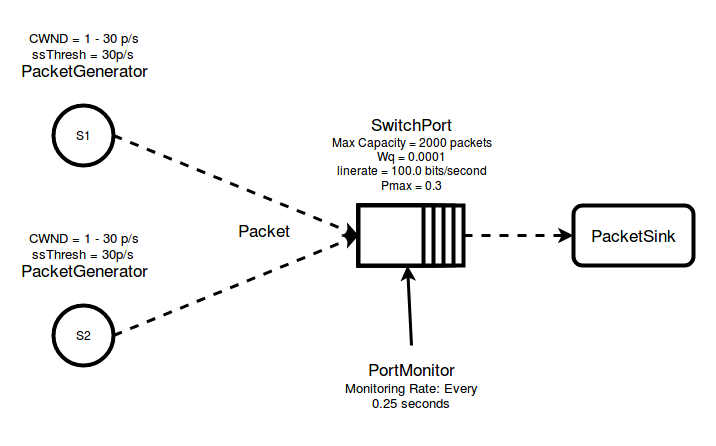
\includegraphics[width = 90mm]{Experiment.png}
	\caption{Sample Experimental Setup}
	\label{fig:exper1}
\end{figure}

Algorithm \ref{alg:2} elaborates the procedure to be undertaken for the training process, and for obtaining the queue table. For every training iteration in the inner loop, we call a function $isGoalState()$ at line 17. This function triggers the call to the simulation, with the weights and other parameters such as buffer size, outbound line rate and maximum CWND threshold indicated in the train function call. Other hyperparameters are also indicated such as number of iterations, learningRate and epsilonDecay. $validMoves$ and $makeMoves$ are functions which return the valid moves from a state and apply a move, respectively. After a call to $isGoalState$, the simulation is run as per the parametric specification, and output is returned in terms of the performance measures (CWND, DROP and STD). Using this, the training algorithm determines if the goal state has been reached or not. Finally, the Q table is returned, using which we can find the optimal path to the correct parameters. Also, it should be noted that $Q_{max}$ and $Q_{min}$ are set to begin from the middle of the buffer. 

\begin{algorithm}[]
  \begin{algorithmic}[1]
  \State [Input: $w_q$, $bufSize$, $CWNDthresh1$, $CWNDthresh2$, $nRepetitions$, $learningRate$, $epsilonDecay$, $validMoves$, $makeMove$].  
  \State [Output:  $Q table$]
  \State $epsilon = 1.0$
  \State $Q$ = \{\}
  \ForAll {$n \in nRepetitions$}
        \State {$epsilon *= epsilonDecay$}
        \State {$s = [bufSize/2 + 1, bufSize/2]$}
        \State {$done = False$}
        \State {$step = 0$}
        \ForAll {$True$}
            \State {$step = 1$}
            \State {$move = epsilonGreedy(epsilon, Q, s)$}
            \State {$sNew = makeMoveF(sNew, move)$}
            \If{$s,move$ not in $Q$}
                \State $Q[s,move] = -1$
            \EndIf
            \If{$isGoalState(sNew)$} \Comment {Run the simulation using Qmax, Qmin, get values and see if they are within the goal state}
                \State $Q[s, move] = -1$
                \State $done = True$
            \EndIf
            \Else
                \If{$step > 1$}
                \State $Q[sOld,moveOld] += learningRate * (-1 + Q[s,move] - Q[sOld,moveOld])$
                \EndIf
                \State $sOld, moveOld = s, move$
                \State $s = sNew$
            \EndIf
        \EndFor
  \EndFor
  \State \Return Q
  \end{algorithmic}
  \caption{\textbf{Training Methodology}}
  \label{alg:2}
\end{algorithm}


\section{Results}
\label{sec:analysis}
We ran our experiments with two sources simultaneously sending packets to a sink, through the buffer. Each of the sources has a max threshold value of 30 packets/second, and were programmed to increase their CWDN by one with every ACK (additive increase), till the threshold is reached. After this, once a packet drop is detected, they perform multiplicative decrease. Note, this procedure is not synchronized. Each source individually is able to find out if its packet was dropped. Also, we set the packet buffer to have a maximum capacity of 2000 packets, with a outbound link capable of servicing 12.5 packets a second. This in turn is connected to a sink, which can log the received packet information. The buffer is also monitored every 0.25 seconds. In our experiments, the queue weights were set to 0.002 and max probability to 0.3. The drop probability increases linearly with increase in queue size.

With this set-up, we initially ran the simulation with values of $Q_{max}$ and $Q_{min}$ which would've been similar to manually configured values (i.e. $Q_{max}$ is twice $Q_{min}$). After this, we ran several rounds of simulations using the values obtained through the reinforcement learning paradigm, followed by the comparison.

For the manually configured values, we used $Q_{min}$ = 800 and $Q_{max}$ = 1600, and ran the simulation. From figure \ref{fig:stable1}, we can see that the buffer size increases gradually and stabilizes near the minimum threshold, at around 900 packets. Packet loss was reported to be 44 and the congestion window total size at the end of the simulation was 17.5 packets/second. 

\begin{figure}[ht!]
	\centering
	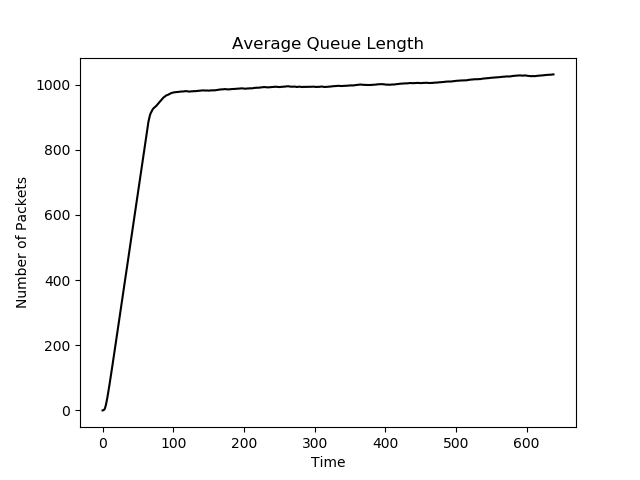
\includegraphics[width = 90mm]{Stable1.png}
	\caption{Queue Stability - Manually Configured Values}
	\label{fig:stable1}
\end{figure}

Now we shall look at the reinforcement learning predicted results. After training for 1000 iterations, with a learning rate of 0.2 and epsilon decay factor of 0.7, and a goal state of CWND > 35, DROP < 20 and STD > 207 the resulting output was $Q_{min}$ = 1738 and $Q_{min}$ = 844. Running the simulation using these values gives us the following results. 

\begin{figure}[ht!]
	\centering
	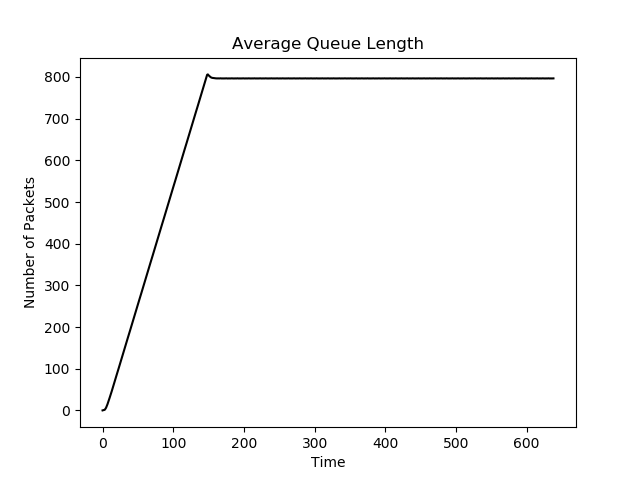
\includegraphics[width = 90mm]{Stable2.png}
	\caption{Queue Stability - Values Determined with Reinforcement Learning}
	\label{fig:stable2}
\end{figure}

The packet loss was predicted to be only 16 packets, and the CWND value was reported to be 37.5. It can be observed from figure \ref{fig:stable2}, that the queue length appears to have stabilized at around 800 packets instead of 1000. This is an improvement, since we desire queue stabilization at lower values (to accommodate bursts). We also observe better values for DROP and CWND, indicating that, reinforcement learning appears to have done better than the manually configured values.

\section{Conclusion}
From the experiments performed, it is clear that a reinforcement-learning based approach is better at finding out optimal values of $Q_{max}$ and $Q_{min}$. The results obtained showed that the queue is capable of not only showing better stability, but also seems to stabilize at a lower values. However, it has to be noted that this only works for a network with characteristics that do not vary much over time. One might argue, considering the dynamic nature of packet-switched networks, that this would mean nothing. However, it is possible to run the training procedure on a constant basis, over several time intervals. 

One other point of contention here has to do with the result itself. It quite clear that we show better results compared to manually configured values, but there's no way by which we guarantee the optimality of the result itself. This is, once again, due to the dynamic nature of packet switched networks, and a degree of uncertainty involved with the probabilistic drop. Further work is necessary to see if a reinforcement-based learning approach is feasible at all.
\label{sec:conc}


\section{Future Work}
\label{sec:future}
This work can be extended in several ways. One, by exploring other control parameters and using mathematical dependencies between them and the network state to our advantage. Two, bringing in a prediction model which is capable of predicting future network states. This would make our current work fit into more dynamic networks. Three, by looking into other techniques such as neural networks and neurofuzzy techniques. And four, trying to perform AQM by modeling the source CWND values as well. 
\bibliographystyle{IEEEtran}
\bibliography{IEEEabrv,bib}

\end{document}